 \documentclass[a4paper,11pt]{article}
\usepackage{fullpage}
\usepackage{amsmath}
\usepackage[boxed]{algorithm}   % drop [boxed] is no box around algorithm wanted
\usepackage[noend]{algorithmic} % drop [noend] if endif, endwhile, etc wanted
\renewcommand{\algorithmiccomment}[1]{\hfill // #1}
\usepackage{graphicx}
\usepackage{listings}
\usepackage{tikz}

\lstdefinelanguage{Python}{
keywords={typeof, null, catch, switch, in, int, str, float, self},
keywordstyle=\color{ForestGreen}\bfseries,
ndkeywords={return,class,if,elif,endif,while, do, else, True, False, def},
ndkeywordstyle=\color{BrickRed}\bfseries,
identifierstyle=\color{black},
sensitive =false,
comment=[1]{\#}
commentstyle=\color{purple}\ttfamily,
stringstyle=\color{red}\ttfamily,
}


\usepackage[
    backend=biber,
    style=ieee,
    sorting=nyt,
    autolang=other
]{biblatex}

\title{\textbf{Software Testing of \\ Numpy Linear Algebra Library\\
        by Team~$7$                                   % Replace t by team number
}
}

\author{Regina \and Suraj \and Johan}  % Replace by your name(s)

    \date{\today}

    \renewcommand{\thesubsection}{\thesection.\Alph{subsection}}


\begin{document}
	\maketitle
	\tableofcontents 
	
\newpage
\section{Introduction}
In this project we develop black and white box tests for Python numpy’s linear algebra package linalg. \\
\\
The project is relevant since numpy linalg is widely used and linear algebra generally can be regarded as an essential scientific field field. Since linear equations are easy to solve many scientific areas include models where equations are approximated using linear equations. Since solutions to equations in many cases are relevant for practical problem solving linear algebra can be very useful, even in its easiest forms. Some areas in which it is used are module theory, representation theory, ring theory, group theory and Galois theory. In functional theory linear algebra is used to study infinite-dimensional problems. In this field many of the analytical solutions break down even though the linear algebra intuition remains. Linear algebra can be used to understand those areas better. \\
\\
The following tools are available through the linalg module in numpy: \\
\\


Core Linear Algebra Tools\\
-------------------------\\
Linear algebra basics:\\
- norm$~~~~~~$             Vector or matrix norm\\
- inv$~~~~~~~$             Inverse of a square matrix\\
- solve$~~~~~$             Solve a linear system of equations\\
- det$~~~~~~~$             Determinant of a square matrix\\
- lstsq$~~~~~$             Solve linear least-squares problem\\
- pinv$~~~~~~$             Pseudo-inverse (Moore-Penrose) calculated using a singular value decomposition\\
- power$~~~~~$    Integer power of a square matrix\\
\\
Eigenvalues and decompositions:\\
- eig$~~~~~~$             Eigenvalues and vectors of a square matrix\\
- eigh$~~~~~$            Eigenvalues and eigenvectors of a Hermitian matrix\\
- eigvals$~~$         Eigenvalues of a square matrix\\
- eigvalsh$~$        Eigenvalues of a Hermitian matrix\\
- qr$~~~~~~~$              QR decomposition of a matrix\\
- svd$~~~~~~$             Singular value decomposition of a matrix\\
- cholesky$~$        Cholesky decomposition of a matrix\\
\\
Tensor operations:\\
- tensorsolve$~~~$     Solve a linear tensor equation\\
- tensorinv$~~~~~$       Calculate an inverse of a tensor\\
\\
Exceptions:\\
- LinAlgError     Indicates a failed linear algebra operation\\

The following linalg functions which we wrote black box tests for: \\
linalg.dot \\
linalg. vdot \\
linalg.inner \\
linalg.outer \\
linalg.matmul \\
linalg.matrix\_power\\
linalg.norm\\
linalg.matrix\_rank\\
linalg.det, slogdet \\
linalg.multidot \\
\\ 
We also wrote white box tests for:\\
linalg.multidot \\




\section{Black-box Testing}
\subsection{linalg.dot}
\subsubsection{documentation}
For 2-D arrays it is equivalent to matrix multiplication, and for 1-D arrays to inner product of vectors (without complex conjugation). For N dimensions it is a sum product over the last axis of a and the second-to-last of b:

    \begin{equation} dot(a, b)[i,j,k,m] = sum(a[i,j,:] * b[k,:,m]) \end{equation}
    
   \paragraph{Paramaters}: \textbf{a} : \textit{array\_like} First argument.\\
	\indent \hspace{2.2cm} \textbf{b} : \textit{array\_like} Second argument.\\
\indent \hspace{2.2cm} \textbf{out} : \textit{ndarray, optional} Output argument. This must have the exact kind that would be returned if it was not used. In particular, it must have the right type, must be C-contiguous, and its dtype must be the dtype that would be returned for dot(a,b). This is a performance feature. Therefore, if these conditions are not met, an exception is raised, instead of attempting to be flexible.
    \paragraph{Returns}:    \textbf{output} : \textit{ndarray}
Returns the dot product of a and b. If a and b are both scalars or both 1-D arrays then a scalar is returned; otherwise an array is returned. If out is given, then it is returned.\\

\paragraph{Raises}:
\textbf{ValueError}
If the last dimension of a is not the same size as the second-to-last dimension of b.

\subsubsection{Tests}
In order to test this function, the input space is partitioned into three types of test suites:

\begin{itemize}
	\item \textbf{Corner cases:} For the corner cases we try to check what happens when dot product is presented with empty arrays.
	
	\item \textbf{Basic properties of the dot-product:} This set of tests ensure that the \textit{dot} function obeys the following mathematical properties.
	\begin{itemize}
		\item[1.] Commutativity: $ a \bullet b = b \bullet a $ 
		\item[2.] Linear: $ a \bullet (\textbf{r}b + c) = \textbf{r}(a \bullet b) + (a \bullet c) $
		\item[3.] Zero dot-product: $ a \bullet 0 = 0 $
		\item[4.] Square of product: $ a \bullet a = | a^2 |$
		\item[5.] Perpendicular vectors: $ c \bullet d = 0$
	\end{itemize}
	
	\item \textbf{Raises case:} This test is setup to ensure that a ValueError is raised when multiplying vectors of different dimensionality.
\end{itemize}

\subsection{linalg.multidot}
Compute the dot product of two or more arrays in a single function call, while automatically selecting the fastest evaluation order.

multi\_dot chains numpy.dot and uses optimal parenthesization of the matrices [R44] [R45]. Depending on the shapes of the matrices, this can speed up the multiplication a lot.

If the first argument is 1-D it is treated as a row vector. If the last argument is 1-D it is treated as a column vector. The other arguments must be 2-D.

\subsubsection{Tests}

\subsection{linalg.vdot}

\subsubsection{documentation}
Return the dot product of two vectors.

The vdot(a, b) function handles complex numbers differently than dot(a, b). If the first argument is complex the complex conjugate of the first argument is used for the calculation of the dot product.

Note that vdot handles multidimensional arrays differently than dot: it does not perform a matrix product, but flattens input arguments to 1-D vectors first. Consequently, it should only be used for vectors.

\paragraph{Paramaters}:	
\textbf{a} : \textit{array\_like} If a is complex the complex conjugate is taken before calculation of the dot product.

\indent \hspace{2.3cm}\textbf{b} : \textit{array\_like} Second argument to the dot product.

\paragraph{Returns}:	
\indent \hspace{0.1cm}\textbf{output} : \textit{ndarray} Dot product of a and b. Can be an int, float, or complex depending on the types of a and b.



\subsubsection{Tests}

For the \textit{vdot} function the input space is partitioned into tests that are formed based on the following division:

\begin{itemize}
	\item \textbf{Basic functionality checks:} These tests involve some regression tests that ensure that the \textit{vdot} function works as intended.
	
	\item \textbf{Complex numbers:} Some tests work with complex numbers to check commutative and square functionlity of the \textit{vdot} function.
	
	\item \textbf{Special cases:} The \textit{vdot} function is checked with floats, empty arrays and negative numbers.
\end{itemize}


\subsection{linalg.inner}
\subsubsection{documentation}
Inner product of two arrays. Ordinary inner product of vectors for 1-D arrays (without complex conjugation), in higher dimensions a sum product over the last axes.

\paragraph{Paramaters}:
\textbf{a}, \textbf{b} : \textit{array\_like} If a and b are nonscalar, their last dimensions must match.

\paragraph{Returns}: \textbf{out} : \textit{ndarray} \textit{out.shape = a.shape[:-1] + b.shape[:-1]}

\paragraph{Raises}:	
\textbf{ValueError} If the last dimension of a and b has different size.
\subsubsection{Tests}
In order to test the \textit{inner} product functionality the test suite is divided based on:

\begin{itemize}
	\item \textbf{Regression Tests:} These tests involve some regression tests that ensure that the \textit{inner} function works as intended.
	
	\item \textbf{Properties of \textit{inner} product:} The inner dot function according to mathworld \footnote{http://mathworld.wolfram.com/InnerProduct.html} should obey the following properties:
	
	\begin{itemize}
		\item[1.] $ \langle u + v,w \rangle = \langle u , w \rangle + \langle v , w \rangle $ 
		\item[2.] $ \langle \alpha~v,w \rangle = \alpha \langle v , w \rangle $
		\item[3.] $ \langle v,w \rangle = \langle w, v \rangle $
		\item[4.] $ \langle v,v \rangle \leq 0 $
		\\
		\\ where $ u, v, w $ are vectors and $ \alpha $ is a scalar.
	\end{itemize}
	
	The first suite of tests check to see how the function behaves when a \emph{zero} case is introduced in the arguments and also if the function works with \emph{float} values. The second suite of tests check whether the \emph{inner} dot product verifies with the properties.
	
	
\end{itemize}

\subsection{linalg.outer}
\subsubsection{documentation}
Compute the outer product of two vectors.

\paragraph{Parameters}:	
\textbf{a} : (M,) \textit{array\_like} First input vector. Input is flattened if not already 1-dimensional.

\textbf{b} : (N,) \textit{array\_like} Second input vector. Input is flattened if not already 1-dimensional.

\textbf{out} : (M, N) \textit{ndarray, optional} A location where the result is stored

\paragraph{Returns}: \textbf{out} : (M, N) \textit{ndarray} \textit{out[i, j] = a[i] * b[j]}


\subsubsection{Tests}

The \emph{outer} product of two vectors behaves as shown below, given two vectors a = [a0, a1, ..., aM] and b = [b0, b1, ..., bN]. The outer product computes :
\newline [[a0*b0 a0*bN... a0*bN]
[a1*b0 ... ] \newline
[~.~~~~~~~~~~~~~~~~~~~~~~~~~~~~~~~~~~~~~~~~~~      ] \newline
[aM*b0...~~~~~~~~~~~~~~~~~~~~~~ aM*bN]] \newline

In order to test the \textit{outer} function tests have been made to check the following:

\begin{itemize}
	\item \textbf{Regression Tests:}  This test sets up a regression test that checks that the \emph{outer} product works as intended with a basic example that verifies the behaviour of the function. 
	\item \textbf{Corner Test:} In order to check the case where the provided vector consists of zero's.
	\item \textbf{Complex value Test: } Since, the documentation claims to also handle complex valued vectors this case makes an \emph{outer} product of two complex valued vectors.
	\item \textbf{Dimension Test:} This test attempts to check how the \emph{outer} product handles vectors of varying sizes.
\end{itemize}

\subsection{linalg.matmul}
\subsubsection{documentation}
Matrix product of two arrays.\\ The behavior depends on the arguments in the following way.\\

If both arguments are 2-D they are multiplied like conventional matrices.\\ If either argument is N-D, N $ > $ 2, it is treated as a stack of matrices residing in the last two indexes and broadcast accordingly.\\ If the first argument is 1-D, it is promoted to a matrix by prepending a 1 to its dimensions. After matrix multiplication the prepended 1 is removed.\\ If the second argument is 1-D, it is promoted to a matrix by appending a 1 to its dimensions. After matrix multiplication the appended 1 is removed.\\ Multiplication by a scalar is not allowed, use * instead. Note that multiplying a stack of matrices with a vector will result in a stack of vectors, but matmul will not recognize it as such.\\


\paragraph{Parameters}:	
\textbf{a} : \textit{array\_like} First argument.

\textbf{b} : \textit{array\_like} Second argument.

\textbf{out} : \textit{ndarray, optional} Output argument. This must have the exact kind that would be returned if it was not used. In particular, it must have the right type, must be C-contiguous, and its dtype must be the dtype that would be returned for dot(a,b). This is a performance feature. Therefore, if these conditions are not met, an exception is raised, instead of attempting to be flexible.

\paragraph{Returns}:	
\textbf{output} : \textit{ndarray} Returns the dot product of a and b. If a and b are both 1-D arrays then a scalar is returned; otherwise an array is returned. If out is given, then it is returned.

\paragraph{Raises}:	\textbf{ValueError} If the last dimension of a is not the same size as the second-to-last dimension of b. If scalar value is passed.

\subsubsection{Tests}



In order to test the \textit{matmul} function tests have been made to check the following:

\begin{itemize}
	\item \textbf{Regression Tests:} This test checks that the function works as intended.
	\item \textbf{Commutative and Distributive Tests:}  These tests ensure that the \textit{matmul} function according to mathworld \footnote{http://mathworld.wolfram.com/MatrixMultiplication.html} obeys properties of commutativity and distributivity.
	\item \textbf{Identity Test:} An identity matrix is multiplied with another matrix to check if the matrix is preserved on matrix multiplication.
	\item \textbf{Raises Checks:} Two tests are setup to ensure that a ValueError is raised when multiplying vectors of different dimensionality and a matrix and scalar are multiplied.
\end{itemize}


\subsection{linalg.matrix\_power}
\subsubsection{documentation}
Raise a square matrix to the (integer) power n.\\ For positive integers n, the power is computed by repeated matrix squarings and matrix multiplications. If n == 0, the identity matrix of the same shape as M is returned. If n < 0, the inverse is computed and then raised to the abs(n).


\paragraph{Parameters}: \textbf{M} : \textit{ndarray or matrix object} Matrix to be “powered.” Must be square, i.e. M.shape == (m, m), with m a positive integer.

\textbf{n} : \textit{int} The exponent can be any integer or long integer, positive, negative, or zero.

\paragraph{Returns}: \textbf{M**n} : \textit{ndarray or matrix object} The return value is the same shape and type as M; if the exponent is positive or zero then the type of the elements is the same as those of M. If the exponent is negative the elements are floating-point.

\paragraph{Raises}:	\textbf{LinAlgError} If the matrix is not numerically invertible.

\subsubsection{Tests}
In order to test the \textit{matrix power} function tests have been made to check the following:

\begin{itemize}
	\item \textbf{Regression Tests:} This test ensures that the matrix when powered by a $ num  geq  1 $ works as intended.
	\item \textbf{Matrix Identity Tests:} This test ensures that a matrix powered by $ num  ==  0 $ produces an identity matrix of the same size. 
	\item \textbf{Matrix Negative Power Check:} This test checks the \emph{matrix power} fuction when $ num  \leq  -1 $.
\end{itemize}
%\subsection{linalg.kron}
%\subsubsection{documentation}



\subsection{linalg.norm}
\subsubsection{documentation}
Matrix or vector norm.

This function is able to return one of eight different matrix norms, or one of an infinite number of vector norms (described below), depending on the value of the ord parameter.\\

\paragraph{Paramaters}: 
x : array\_like
Input array. If axis is None, x must be 1-D or 2-D.
ord : {non-zero int, inf, -inf, ‘fro’, ‘nuc’}, optional
Order of the norm (see table under Notes). inf means numpy’s inf object.
axis : {int, 2-tuple of ints, None}, optional
If axis is an integer, it specifies the axis of x along which to compute the vector norms. If axis is a 2-tuple, it specifies the axes that hold 2-D matrices, and the matrix norms of these matrices are computed. If axis is None then either a vector norm (when x is 1-D) or a matrix norm (when x is 2-D) is returned.
keepdims : bool, optional
If this is set to True, the axes which are normed over are left in the result as dimensions with size one. With this option the result will broadcast correctly against the original x.
New in version 1.10.0.\\

\paragraph{Returns}:    
n : float or ndarray
Norm of the matrix or vector(s).\\

\subsubsection{tests}


\subsection{linalg.matrix\_rank}
\subsubsection{documentation}
Return matrix rank of array using SVD method
Rank of the array is the number of singular values of the array that are
greater than `tol`.
\paragraph{Paramaters}:  M : {(M,), (..., M, N)} array\_like input vector or stack of matrices
tol : (...) array\_like, float, optional
threshold below which SVD values are considered zero. If `tol` is None, and ``S`` is an array with singular values for `M`, and ``eps`` is the epsilon value for datatype of ``S``, then `tol` is set to ``S.max() * max(M.shape) * eps`` Broadcasted against the stack of matrices hermitian : bool, optional If True, `M` is assumed to be Hermitian (symmetric if real-valued),
enabling a more efficient method for finding singular values. Defaults to False.
\paragraph{Returns}: 
\subsubsection{tests}
test\_simple\_case: a simple 3X3 eye matrix is tested \\
\\
test\_scalar: the rank of a scalar input equates to 1. \\
\\
test\_array: same as above but a scalar inside an array. \\
\\
test\_zero\_rank: the rank of a matrix with zeros will equate to 0. \\
\\
test\_1\_dimensional\_matrix: the rank of a 1 dimensinal matrix should be 1. \\
\\
These tests were written to test the functionality of matrix rank with various simple integer inputs. 


\subsection{linalg.det, linalg.slogdet}
\subsubsection{documentation}
Determinants are used to define the characteristic polynomial of a matrix and whether it has a unique solution or not. This function computes the sign and (natural) logarithm of the determinant of an array. A number representing the sign of the determinant. For a real matrix,
this is 1, 0, or -1. For a complex matrix, this is a complex number with absolute value 1 (i.e., it is on the unit circle), or else 0. The determinant is computed via LU factorization using the LAPACK
routine z/dgetrf. The determinant of a 2-D array ``[[a, b], [c, d]]`` is ``ad - bc``. (sign, logdet) = np.linalg.slogdet(a)
\paragraph{Paramaters}: An array or matrix with single, double, complex single or complex double type. 
\paragraph{Returns}: A scalar. 
\subsubsection{tests}
test\_det: This tests that the determinant calculation works according to the above. \\
\\
test\_size\_zero: This tests that the sign of the determinant an empty matrix is a complex number and that the determinant itself is 1. \\
\\
test\_types: This tests that the output type of the determinant is the same as the input type, i.e. single, double, csingle and cdouble. \\
\\
These tests were written to test matrix determinants with various simple inputs. The determinant function was also evaluated with double, complex single and complex double datatypes. 

\subsection{linalg.multidot (Black box tests)}
\subsubsection{documentation}
Compute the dot product of two or more arrays in a single function call, while automatically selecting the fastest evaluation order. `multi\_dot` chains `numpy.dot` and uses optimal parenthesization of the matrices. Depending on the shapes of the matrices, this can speed up the multiplication a lot. If the first argument is 1-D it is treated as a row vector. If the last argument is 1-D it is treated as a column vector. The other arguments must be 2-D.\\
\\
TestCases: Test cases are created so that vectors when multiplied share the same dimensions. When matrices are multiplied they need to be organized so that the first dimension of the first matrix is the same as the second dimension of the second matrix etc. 
\paragraph{Paramaters}: Vectors or matrices. They must be organized so that the first dimension of the first matrix is the same as the second dimension of the second matrix etc. 
\paragraph{Returns}: A vector or matrix whose dimension depends on the inputs. 
\subsubsection{Tests}
test\_three\_inputs\_vectors: This tests the multidot function with three vectors. The assert is the following: assert\_almost\_equal(multi\_dot([A, B]), A.dot(B))\\
\\
test\_three\_inputs\_matrices: This tests the multidot function with three matrices\\
\\
test\_four\_inputs\_matrices: This tests the multidot function with four matrices\\
\\
test\_shape\_vector\_first: This tests the multidot function with a vector with n rows as the first argument followed by three matrices with dimensions n, m and m, n. The shape result sought is the same as the vector, i.e. 1 dimensional with n rows. \\
\\
test\_shape\_vector\_last: This tests the multidot function with a n rows vector as the last argument preceded by three matrices with dimensions m, n and n, m. The shape result sought is m. \\
\\
test\_shape\_vector\_first\_and\_last: This tests the multidot function with n rows vector as the first and last arguments with two matrices with dimensions n, m and m, n in the middle. The shape result sought is () since the result is a scalar. assert\_equal(multi\_dot([A1d, B, C, D1d]).shape, ())\\
\\
test\_types: This runs the test\_three\_inputs\_matrices above using integers, doubles, complex numbers. \\
\\
These tests were written to test the functionality of multidot with various inputs. All test cases are initialized with random values. 

\subsection{Datatype tests}
A separate testclass was created to test linalg functions with various datatypes. The functions were run with values of these datatypes and the output was checked to still be the same datatype. The datatypes used were single, double, complex single and complex double. The functions tested with the datatypes were matrix invariant, eig and eigenvalues for normal and hermitian cases, single value decomposition and determinant.  



\section{White-Box Test}
In this section we aim to use what we can see from the functions themselves to satisfy some coverage
criteria. To evaluate coverage we will use the coverage.py package. This can evaluate both statement and branch coverage and enumerate which statements or branches were not executed.

As our function contains a loop we want to include loop coverage. 

The function we have chosen to white box test is the multi\_dot() function and it's subsidiary functions \_multi\_dot() and multi\_dot\_three().

This function performs the dot product of an array of arrays. It consists of several if/ else statements, a recursive loop and several different return options. In our testing we want to ensure that all statments and edges of length 2 are covered insofar as possible along with coverage of the loops. 



\paragraph{Node Coverage}


For node coverage we have the critereon that our tests cause all statements in the program to be executed. Thus we want to ensure that in our set of tests that all nodes are visited on at least one test path. Figure 1 shows the control flow graph for the functions under test. 



\paragraph{Edge Coverage}
In our tests we endeavour to execute all edges of (up to) length 2. 
For edge coverage we have the critereon that all edges of length two are executed i.e.
we want to ensure that for each decision made all possible next decisions are executed. 
Our test requirements are that every edge of length 2 is contained in at least one of our test paths.
\\
Note: This is not possible given the layout of the code under test for reasons given below in \emph{loop coverage}
\paragraph{Loop Coverage}

A loop is covered if in at least one test executed the loop 0 times, if in some test the loop was executed exactly once, and if in some test the body was executed more than once. 
In the case of this code we can't test it only once so we execute it a minimum number of times i.e. with four arrays.
This is because the function \_multi\_dot is only called when there are more than three arguments. It is a self calling function that iteratively divides the arrays based on a precomputed best order. it stops when the two indices passed are the same so the minimum number of calls is more than one.
This also means that the edge from 8-10-16 cannot be tested.
The test cases that test the loop functionality are 
\begin{itemize}
\item Zero times - Test 1 - The \_multi\_dot function is not called.  
\item Minimum - Test 5.
\item Many times - test 7 - The loop recurses many times
\end{itemize}


To achieve coverage for these cases we create a set of test paths that between them include all nodes and edges of length 2 along with paths that execute the loop zero times, the minimum amount of times and many times. 

\begin{enumerate}
\item \{1,2\}
\item \{(1,3)\} 
\item \{1,4,5,6,8,9,11,13,15,16,18\}
\item \{1,4,6,7,8,9,11,13,14,16,18\}
\item \{1,4,5,6,7,8,10,12,10,16,17\}

\item \{1,4,6,8,9,11,13,14,16,19\}
\item \{1,4,5,6,8,10,12,10,12,10,16,18\}
\item \{1,4,6,8,10,12,10,12,10,16,19\}
\item \{1,4,5,6,7,8,9,11,13,14,16,17\} %% all <2 and C1<C2
\item \{1,4,5,6,7,8,9,11,13,15,16,17\} %dims 1 for 0 & -1 and C1>C2
\item \{1,4,6,8,11,13,15,16,19\} %dims >2 for all and C1>C2


\end{enumerate}
The path \{8,10,16\} cannot be executed due to the reasons given above.

Below we describe the test cases for each test path.

\paragraph{Test Path 1}

To construct a test case for the first path enumerated above we need to pass an array with fewer than 2 arguments. 
The test test\_multi\_dot\_raises was created to execute path 1. It returns a raises value error.


\paragraph{Test Path 2}
To execute path 2 the test test\_multi\_two was created. This path was constructed to have exactly two arguments in the passed array.
This path calls the dot fonction and then returns. It returns the dot product of the two.


\paragraph{Test Path 3}
Test case - test\_multi\_ndim\_end1\\
Test case 3 tests three different branches:\\
\begin{itemize}
\item By setting the number of array arguments to 3 we take the third arm of the first branch which brings us into the main body of the program. by choosing exactly 3 arguments we also test the branch calling the multi\_dot\_three function or the branch from 8-9.
\item By not setting the dimension of the last argument to 1 we do not execute the if statement and instead go from 6-8.
\item By setting the dimesion of the first argument to be 1 we execute the branches 4-5 and 16-18.
\item The ordering of the arguments dictates which branch is taken within the multi\_dot\_three function. The test test\_multi\_ndim\_10 is ordered so that the branch from 13-15 is taken. 
\end{itemize}


%\paragraph{Test 4: Arguments=3,dimension of last argument = 1}
\paragraph{Test path 4}
test case - test\_multi\_ndim\_01\\ 
Test case 3 tests three different branches:\\
\begin{itemize}
\item By setting the dimesion of the last argument to be 1  we execute the if statement branch from  6-7.
\item By not setting the dimension of the first argument to 1 we do not execute the if statement branch from 4-5 and instead go 4-6.
\item The ordering of the arguments dictates which branch is taken within the multi\_dot\_three function. The arguments of test\_multi\_ndim\_01 are ordered so that the branch from 13-14 is taken. 
\end{itemize}



%\paragraph{Test 5: Arguments$>$3,dimension of first and last argument = 1}
\paragraph{Test Path 5}

test case - test\_multi\_ndim\_11\\
Test case 3 tests three different branches:\\
\begin{itemize}
\item By setting the dimesion of the last argument and the last argument to be 1  we execute both if statement branches from 4-5 and  6-7.
\item By having more than 3 arguments we take the branch into the \_multi\_dot fucntion from node 8-10. 
\item By setting the number of arguments to 4 we execute the loop a minimum number of times.   
\item As both the dimesion of the first and last argument are 1 we execute the if statement from 16-17.   
\end{itemize}


\paragraph{Test Path 6} %1-4-6-8-9-11-13-14-16-19

test case - test\_multi\_ndim\_00\\
This path was constructed for the sole purpose of testing he edge of length two from 14-16-19.
The test case was constructed by giving the first and last arguments of the array dimensions greater than 1, and by ordering the arrays within the main array to ensure that C1$<$C2 

%\paragraph{Test 6: Arguments=3,dimension of first and last argument $>$ 1}
\paragraph{Test Path 7}

test case - test\_multi\_ndim\_00\\
This test was created to test the case where neither of the if loops from 4-5 and 6-7 are executed. This also gives that the if statement from 14-16-19 is executed.  


\paragraph{Test Path 7}
test case - test\_many\_ndim\_11\\

This test was created to test the path where the loop 10-12-10 is executed multiple times.

This also gives that the if statement given by the edge 10-16-17 is executed.  


\paragraph{Test path 8}%\item \{1,4,6,8,10,12,10,12,10,16,19\}
test case - test\_many\_ndim\_00\\

This path was constructed solely to test the edge of length two from 10-16-19. to do this we ensure that the first and last arguments do not have dimesion of 1.

\paragraph{Test path 9}%\item \{1,4,5,6,7,8,9,11,13,14,16,17\} %% all <2 and C1<C2

Test case - test\_3\_C1\_00
This path was constructed solely to test the edge of length two from 14-16-17. to do this we ensure that the first and last arguments have dimesionality of 1 and that C1$<$C2.

\paragraph{Test path 10}%\item \{1,4,5,6,7,8,9,11,13,15,16,17\} %dims 1 for 0 & -1 and C1>C2
Test case - test\_3\_C2\_11

This path was constructed to test only the edge of length two from 15-16-17. to do this we ensure that the first and last arguments have dimesionality of 1 and that C1$>$C2.

\paragraph{Test path 11}%\item \{1,4,6,8,11,13,15,16,19\} %dims >2 for all and C1>C2
Test case - test\_3\_C2\_00

This path was constructed to test only the edge of length two from 15-16-19. to do this we ensure that the first and last arguments do not have dimesion of 1 and that C1$>$C2.

  \begin{tikzpicture}[%
    ->,
    shorten >=2pt,
    >=stealth,
    node distance=1cm,
    noname/.style={%
      circle,
      minimum width=5em,
      minimum height=3em,
      draw
    }
  ]
    \node[noname] (1)                                             {1};
    \node[noname] (2) [below=of 1]                                {2};
    \node[noname] (4) [node distance=1cm and 3mm,below left=of 2] {4};
    \node[noname] (3) [left=of 4]                                 {3};
    \node[noname] (5) [below=of 4]                                {5};
    \node[noname] (6) [node distance=2cm,right=of 5]              {6};

    \path (1) edge                   node {} (2)
          (2) edge                   node {} (3)
          (2) edge                   node {} (4)
          (2) edge                   node {} (6)
          (3) edge                   node {} (5)
          (4) edge                   node {} (5)
          (5) edge [bend right=20pt] node {} (2);
  \end{tikzpicture}







\section{Conclusion}
All the tests developed in this project for certain functions of the numpy linalg package yielded good test results and we therefore conclude that they function properly. All the tests do not cover all the possible input parameter datatypes such as complex numbers, which weakens the suite. Developing such tests in a fully comprehensive manner was found to be difficult due to the various functionalities of the package. Software testing is fun and exciting!

\section{Appendix}

\subsection{whitebox}

\lstinputlisting{whiteBoxTest.py}


\subsection{linalg.dot}
\lstinputlisting{../testdot.py}

\subsection{linalg.vdot}
\lstinputlisting{../testvdot.py}

\subsection{linalg.inner}
\lstinputlisting{../testinner.py}

\subsection{linalg.outer}
\lstinputlisting{../testouter.py}

\subsection{linalg.matmul}
\lstinputlisting{../testmatmul.py}

\subsection{linalg.matrixpower}
\lstinputlisting{../testmatrixpower.py}

\subsection{test\_multi\_dot}	
\begin{figure}[H]
	\centering
	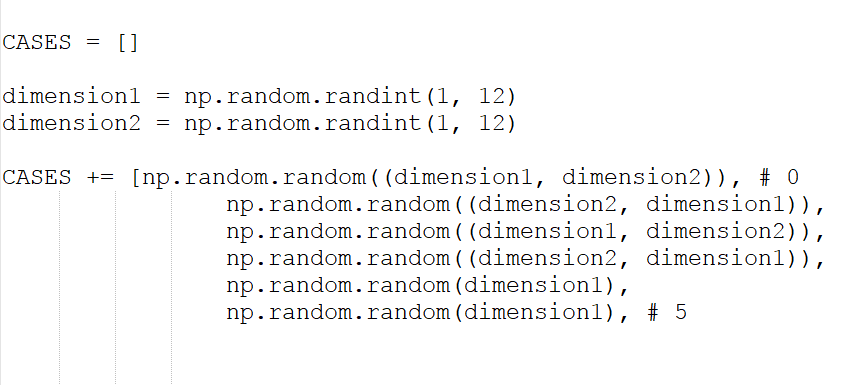
\includegraphics[width=0.6\textwidth]{snippets/multi_dot/1CASES.PNG}
	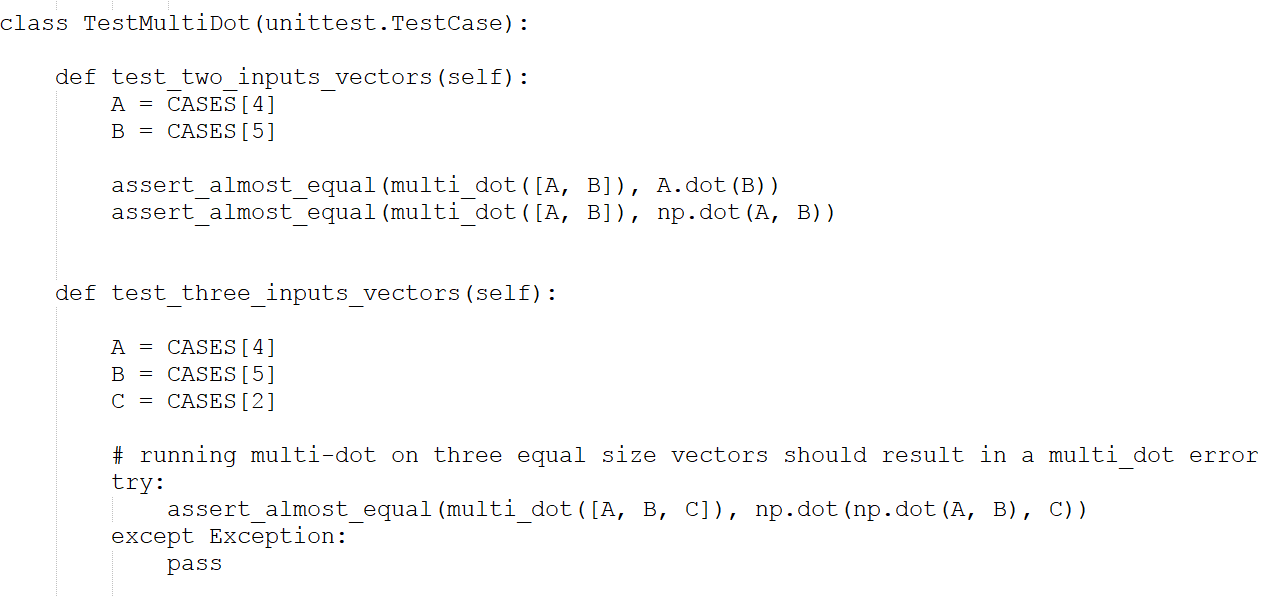
\includegraphics[width=0.6\textwidth]{snippets/multi_dot/2.PNG}
	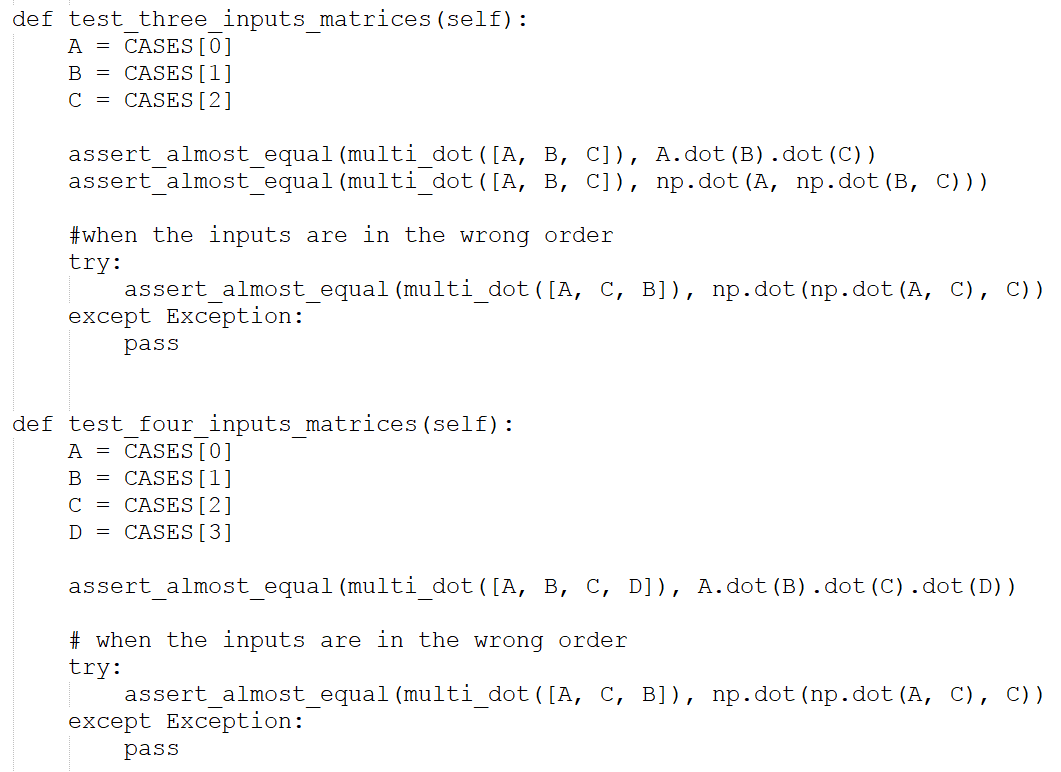
\includegraphics[width=0.6\textwidth]{snippets/multi_dot/3.PNG}
	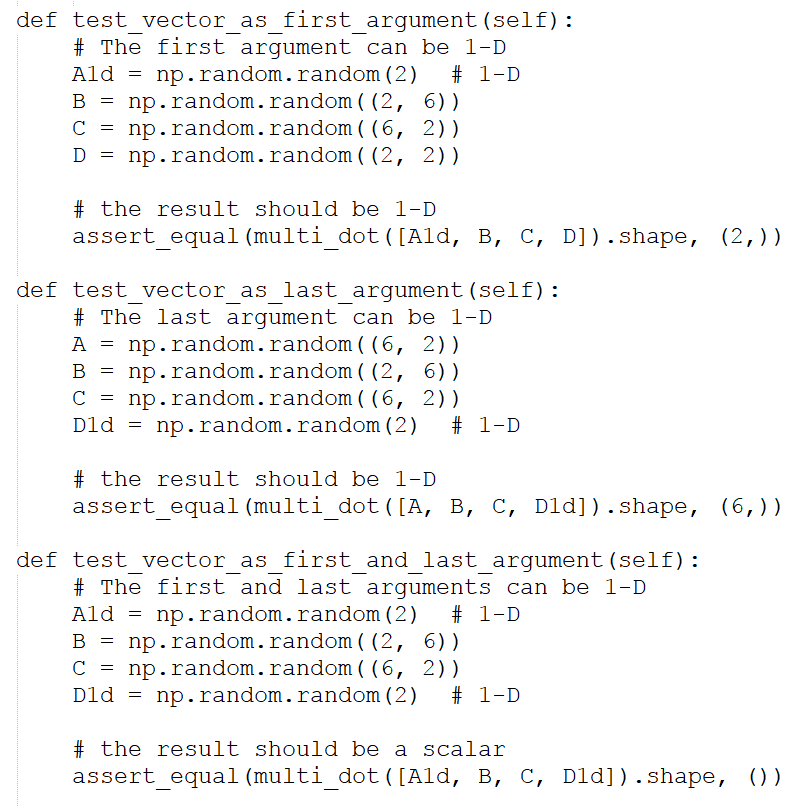
\includegraphics[width=0.5\textwidth]{snippets/multi_dot/4.PNG}

\end{figure}

\subsection{test\_matrix\_rank}	
\begin{figure}[h]
	\centering
	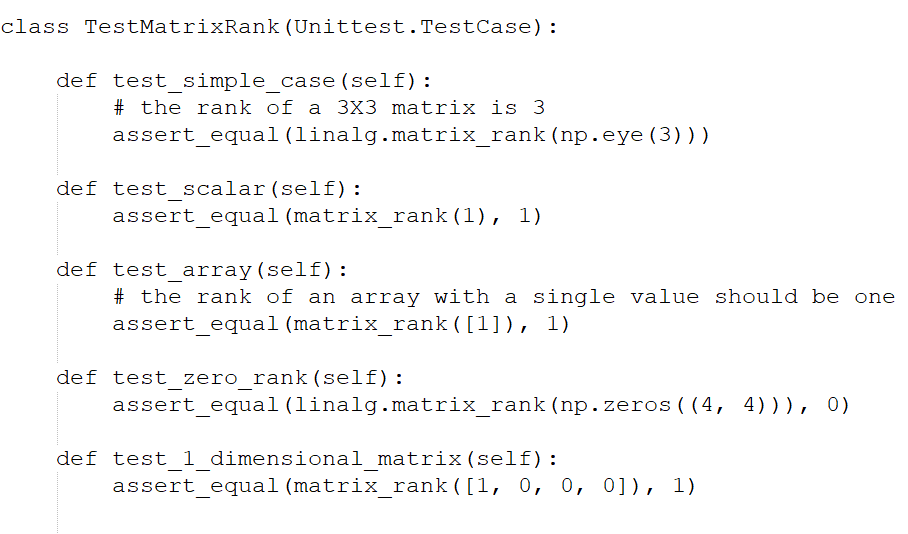
\includegraphics[width=0.70\textwidth]{snippets/rank/1.PNG}
\end{figure}

\subsection{test\_matrix\_determinant}	
\begin{figure}[h]
	\centering
	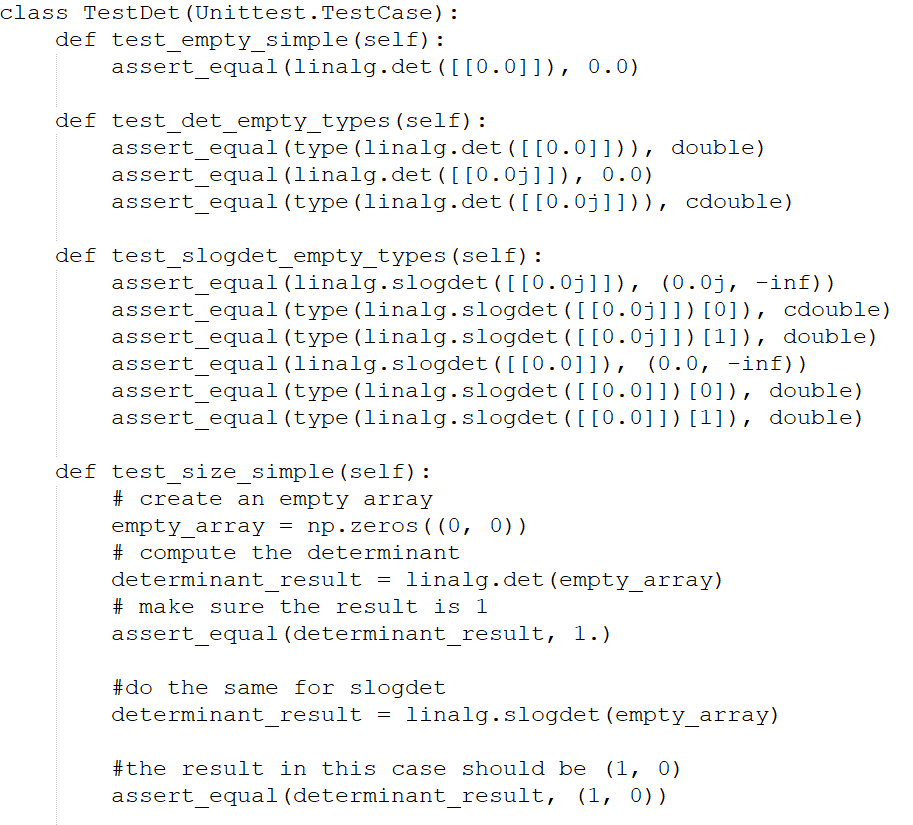
\includegraphics[width=0.70\textwidth]{snippets/Det/1.PNG}
\end{figure}

\subsection{test\_datatypes}	
\begin{figure}[h]
	\centering
	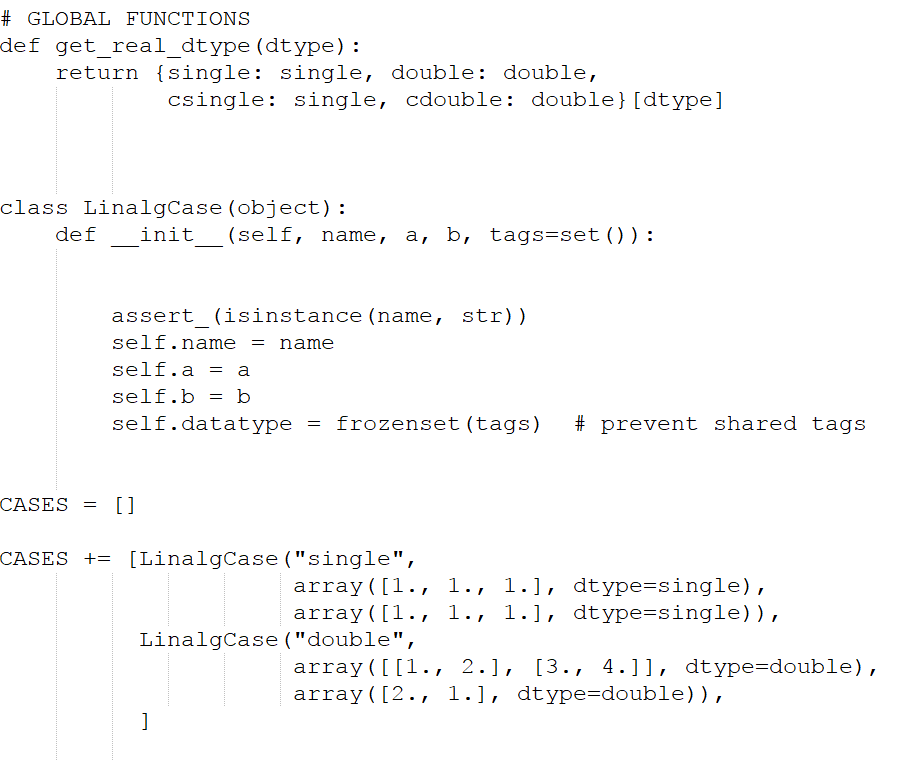
\includegraphics[width=0.70\textwidth]{snippets/datatypes/2.PNG}
	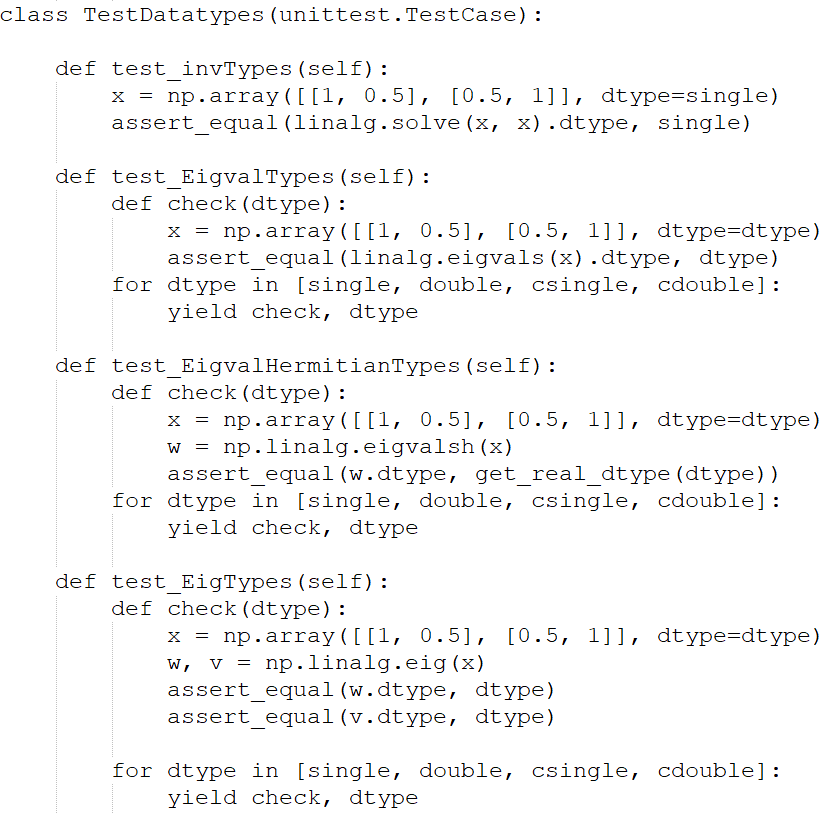
\includegraphics[width=0.70\textwidth]{snippets/datatypes/3.PNG}
	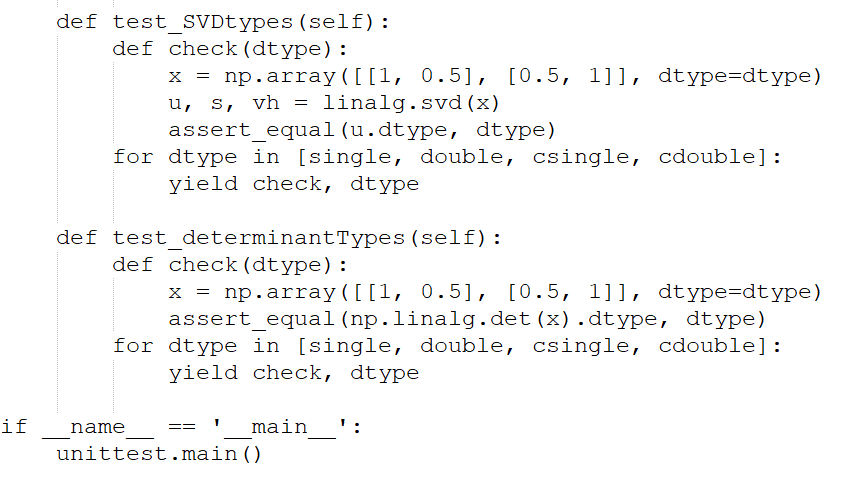
\includegraphics[width=0.70\textwidth]{snippets/datatypes/4.PNG}
\end{figure}

\newpage	
\end{document}
